\section{General Discussion}

The results suggest that, for visual searches involving locating a target on an otherwise homogeneous surface texture, human behaviour can be modelled closely by a stochastic process. The random walk model finds the target in a similar number of fixations as a typical human observer and produces scan-paths that are spatially distributed in a similar way to human scan-paths. The random walk model also makes a similar number of re-fixations and, except for the initial few fixations, searches as efficiently as human observers. 
\par
However, this is not to say that our results challenge Guided Search: in fact the two models could quite easily work together. In fact, the model presented in this paper \itshape is \normalfont guided. When the target is salient against the textured background then the model is likely to make a saccade to that location. One could imagine that if there are several search items that could potentially be the target, as there are in most typical visual search experiments, that a random walk model could be used to choose which item should be fixated next. Also, although our model did not need any form of memory or inhibiton of return, we do not mean to suggest that there is no inhibition of return in any form of human search. Indeed, as our stimuli contain no search objects, any IoR process would have to be operating with respect to spatial coordinates defined with respect to the stimulus boundaries, rather than being applied to discrete search objects. However, as we can see from Figure \ref{fig:refixations} human observers do not appear to re-fixate recently fixation regions any more or less than we would expect a stochastic, memory-less process to. Further research and experiments would be needed to characterise this behaviour more thoroughly. 
\par
This is a somewhat surprising result given that \cite{najemnik-geisler2008} have shown that human observers appear to be near optimal in their search strategy. Najemnik and Geisler also compared the spatial distributions of the fixations chosen by their ideal observer, a MAP model, and human subjects, and found that both human subjects and the ideal observer show a clear preference for fixation on small regions above and below the centre of the image. However, there is no evidence for this distribution in our data, which show no preferences for fixating any particular regions (see Figure \ref{fig:hotspot}). 

\par

There have been a series of papers using Classification Images to investigate guidance in a search task involving targets embedded in $1/f$-noise \citep{rajashekar2002, rajashekar2006, tavassoli2009}. This involves recording all the fixation locations and computing the mean region that is fixated on. For a search task involving a geometric shape embedd in $1/f$ noise, these classification images have been shown to resemble the target which is being searched for. However theses results do not appear to hold when the analysis methods are applied to the data from \cite{clarke2009}. The classification images obtained from the seven observers are shown in Figure \ref{fig:CIresults}. This could be because either guidance does not play a significant role with these stimuli or, due to the the small size of the target, there is a larger degree of variance in fixation placement with respect to the intended point of interest. This means that even if the observers were directing their attention to regions of the surface that resembled the target, they would be unlikely to be visible in the classification images. 

It could be that the target is too small when compared to the background and does not show up due to spatial uncertainties (need a better way of saying this). 

\begin{figure*}
	\centering
		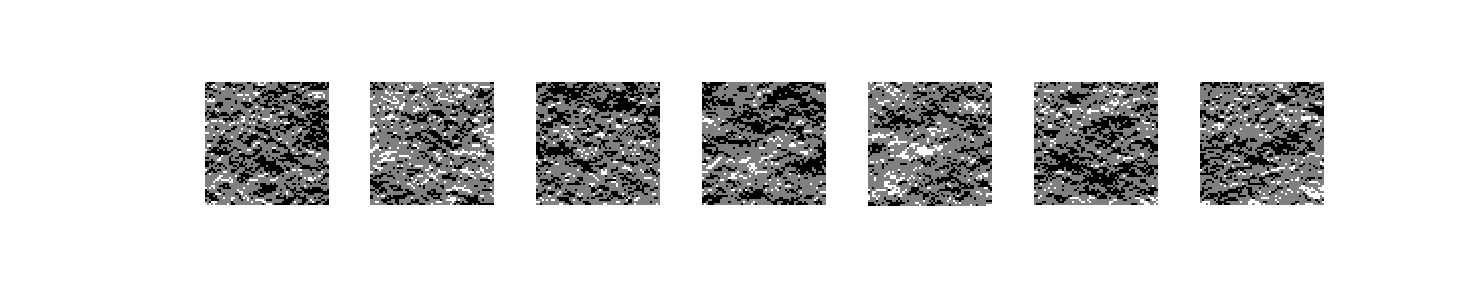
\includegraphics[width=14cm]{figures/CIresults.eps}
	\caption{Classification Images obtained for each of the seven observers in the first visual search experiment in \cite{clarke2009}}
	\label{fig:CIresults}
\end{figure*}

\subsection{Conclusions}
As stated above, a complete, computational visual search model should possess two parts: a feature extraction front end and a search strategy. The aim of this paper was to explore to what extent a search strategy based on a random walk could account for human performance. Previously implemented search strategies have generally worked in a serial manner, checking items one at a time, with some form of imperfect memory \citep{melloy2006, rutishauser-koch2007}. One search model that makes use of parallel target detection over a serial sequence of fixations is the Ideal Observer. One problem with this approach is that it assumes that the target will be located at one of a predefined independent finite number of potential target locations. Unfortunately, this assumption breaks down when image processing techniques are used, as the activation at any pixel is likely to be correlated with its neighbours. Hence we have explored an alternative explanation of human search strategies: a random walk. While the use of a random walk to explain patterns of fixations is not new \citep{greene2008, aks2002, morawski1980}, our model is unlike earlier ones in being strongly based on empirical data. We find that a random walk behaves in a similar way to human observers, both in terms of the number of saccades required to find the target, and the spatial distribution of fixations. 
\par
Our results here suggest that inhibition of return; integration of information across fixations, and more general memory based processes do not have a large role to play in at least one type of search task (search for an inconspicuous target on a continuously textured surface). Future testing of models of visual search should consider not only possible differences between search strategies on different types of stimuli, but also variation between observers in their strategies. It may be possible to obtain evidence for more than one model of search strategy depending on the observers tested.
